\documentclass[tikz]{standalone}

\usepackage{fontawesome}

\usetikzlibrary{positioning}

\begin{document}
	\begin{tikzpicture}[
		block/.style={draw, very thick, fill=white, minimum height=18ex, minimum width=8em, text width=8em, align=center},
		super block/.style={draw, very thick, fill=white, minimum height=10ex, minimum width=32em, align=center},
	]
		\coordinate (in) at (0,0);
		\node [block, right=of in] (comm) {\faKey\\Communication\\and\\security};
		\node [block, right=of comm] (comp) {\faCalculator\\Computation\\and\\simulation};
		\node [block, right=of comp] (sens) {\faCompass\\Sensing\\and\\metrology};
		\coordinate[right=of sens] (out);

		\node [super block, below=of comp] {Basic science};
		\node [super block, above=of comp] {Application};
	\end{tikzpicture}
\end{document}
